\documentclass{pssbmac}

%%%%%%%%%%%%%%%%%%%%%%%%%%%%%%%%%%%%%%%%%%%%%%%%%%%%%%%%%%%%%%%%%%%%%%%%
%% POR FAVOR, NÃO FAÇA MUDANÇAS NESSE PADRÃO QUE ACARRETEM  EM
%% ALTERAÇÃO NA FORMATAÇÃO FINAL DO TEXTO
%%%%%%%%%%%%%%%%%%%%%%%%%%%%%%%%%%%%%%%%%%%%%%%%%%%%%%%%%%%%%%%%%%%%%%%%

%%%%%%%%%%%%%%%%%%%%%%%%%%%%%%%%%%%%%%%%%%%%%%%%%%%%%%%%%%%%%%%%%%%%%%%%
% POR FAVOR, ESCOLHA CONFORME O CASO
%%%%%%%%%%%%%%%%%%%%%%%%%%%%%%%%%%%%%%%%%%%%%%%%%%%%%%%%%%%%%%%%%%%%%%%%
%\usepackage[brazil]{babel} % texto em Português
\usepackage[english]{babel} % texto em Inglês

%\usepackage[latin1]{inputenc} % acentuação em Português ISO-8859-1
\usepackage[utf8]{inputenc} % acentuação em Português UTF-8
%%%%%%%%%%%%%%%%%%%%%%%%%%%%%%%%%%%%%%%%%%%%%%%%%%%%%%%%%%%%%%%%%%%%%%%%


%%%%%%%%%%%%%%%%%%%%%%%%%%%%%%%%%%%%%%%%%%%%%%%%%%%%%%%%%%%%%%%%%%%%%%%%
%% POR FAVOR, NÃO ALTERAR
%%%%%%%%%%%%%%%%%%%%%%%%%%%%%%%%%%%%%%%%%%%%%%%%%%%%%%%%%%%%%%%%%%%%%%%%
\usepackage[T1]{fontenc}
\usepackage{float}
\usepackage{graphics}
\usepackage{graphicx}
\usepackage{epsfig}
\usepackage{indentfirst}
\usepackage{amsmath, amsfonts, amssymb, amsthm, mathtools}
\usepackage{url}
\usepackage{csquotes}
\usepackage{lipsum}
% Ambientes pré-definidos
\newtheorem{theorem}{Theorem}[section]
\newtheorem{lemma}{Lemma}[section]
\newtheorem{proposition}{Proposition}[section]
\newtheorem{definition}{Definition}[section]
\newtheorem{remark}{Remark}[section]
\newtheorem{corollary}{Corollary}[section]
\newtheorem{teorema}{Teorema}[section]
\newtheorem{lema}{Lema}[section]
\newtheorem{prop}{Proposi\c{c}\~ao}[section]
\newtheorem{defi}{Defini\c{c}\~ao}[section]
\newtheorem{obs}{Observa\c{c}\~ao}[section]
\newtheorem{cor}{Corol\'ario}[section]

% ref bibliográficas
\usepackage[backend=biber, style=numeric-comp, maxnames=50]{biblatex}
\addbibresource{refs.bib}
\DeclareTextFontCommand{\emph}{\boldmath\bfseries}
\DefineBibliographyStrings{brazil}{phdthesis = {Tese de doutorado}}
\DefineBibliographyStrings{brazil}{mathesis = {Disserta\c{c}\~{a}o de mestrado}}
\DefineBibliographyStrings{english}{mathesis = {Master dissertation}}
%%%%%%%%%%%%%%%%%%%%%%%%%%%%%%%%%%%%%%%%%%%%%%%%%%%%%%%%%%%%%%%%%%%%%%%%


\begin{document}

%%%%%%%%%%%%%%%%%%%%%%%%%%%%%%%%%%%%%%%%%%%%%%%%%%%%%%%%%%%%%%%%%%%%%%%%
% TÍTULO E AUTORAS(ES)
%%%%%%%%%%%%%%%%%%%%%%%%%%%%%%%%%%%%%%%%%%%%%%%%%%%%%%%%%%%%%%%%%%%%%%%%

\title{Topological characteristics of the road network in São Paulo, Brazil}

\author{
    {\large Pedro Augusto Borges dos Santos}\thanks{pedro.borges@inpe.br},\  {\large Dr. Leonardo Bacelar Lima Santos}\thanks{leonardo.bacelar@inpe.br}\\
    {\small Instituto Nacional de Pesquisas Espaciais, São José dos Campos, SP}
}
\criartitulo
%%%%%%%%%%%%%%%%%%%%%%%%%%%%%%%%%%%%%%%%%%%%%%%%%%%%%%%%%%%%%%%%%%%%%%%%


%%%%%%%%%%%%%%%%%%%%%%%%%%%%%%%%%%%%%%%%%%%%%%%%%%%%%%%%%%%%%%%%%%%%%%%%
% TEXTO
%%%%%%%%%%%%%%%%%%%%%%%%%%%%%%%%%%%%%%%%%%%%%%%%%%%%%%%%%%%%%%%%%%%%%%%%

\begin{abstract}

Road networks are critical infrastructure systems that can be severely disrupted by natural or human-made events, making the analysis of their structural properties essential for urban planning and emergency management. This study investigates the topological characteristics of the road network of São Paulo, Brazil. Four graph-based metrics were computed: node degree ($k_i$), node clustering coefficient ($c_i$), node average shortest path length ($l_i$), and edge betweenness centrality ($e_{ij}$). Additionally, the network was compared to an equivalent random graph $G(N, p)$ to assess its structural properties. The network was modeled as a directed multigraph with 122,456 nodes and 304,027 edges. Results show that the degree distribution does not follow a power-law behavior, indicating the network is not scale-free, with most intersections having a degree value of 6. A small subset of edges concentrates high $e_{ij}$ values, identifying critical road segments whose failure could significantly disrupt connectivity across the city. Compared to an equivalent random graph, the real network presents a substantially higher clustering coefficient and an average shortest path length approximately 18 times larger, reflecting the geographical constraints inherent to physical road infrastructure. These findings contribute to understanding the structural vulnerability of São Paulo's road network and provide a foundation for future resilience analyses.

\noindent
{\bf Keywords}. urban road network, complex networks, network topology, edge betweenness centrality, São Paulo
\end{abstract}

\section{Introduction}

Road networks are vulnerable to disasters, which can cause damage to the infrastructure and adversely affect travel on the degraded network. Additionally, human-made events such as road crashes and road maintenance can affect road serviceability. After such events, certain places often become less accessible. Studying and analyzing the topological characteristics of road networks helps prioritize planning, budgeting, and maintenance, as well as preparing effective emergency response plans \cite{balijepalliMeasuringVulnerabilityRoad2014}.

Although the literature on road network vulnerability has advanced in proposing metrics and methodologies, it is not yet fully clear how these structural properties behave in specific urban contexts. Each city has its own characteristics of road design, intersection density, and mobility patterns, which can directly influence graph measures. Understanding how these properties manifest in the studied spatial context is essential to reveal potential particularities that may guide local policies for planning and managing road infrastructure.

In this context, the objective of this study is to analyze the topological characteristics of urban roads in São Paulo, Brazil. The paper includes the analysis of the road network as a graph, with the computation of degree, average shortest path length, clustering, and edge betweenness, to identify potential vulnerabilities in the network.

The characteristics of a road network can be modeled as a graph object. A graph, or a network, is a mathematical structure used to model pairwise relations between entities, regardless of their nature, enabling the analysis of connectivity patterns, structural properties, and dynamic processes across a wide range of domains, from social interactions and biological systems to transportation and urban infrastructure \cite{Newman2010}.

Previous studies have investigated the vulnerability of transport and road networks using graph-based approaches in urban road networks \cite{morelliMeasuringUrbanRoad2021} and rural road networks \cite{santosVulnerabilityAnalysisComplex2023}, analyzing vulnerability to flooding in mobility systems.

\section{Material and methods}

\subsection{Study area}

The area investigated included the complete territory of São Paulo, Brazil. From the selected area, it was possible to load the road network graph from January 2026, using the osmnx Python library \cite{boeingModelingAnalyzingUrban2025}.

\subsection{Graph analysis}

The road network is represented by a graph $G$, where each intersection is a node and each road segment is an edge. Therefore, $V$ is a set of vertices (or nodes) and $E$ is a set of edges (or links) that connects pairs of nodes (or connects a node to itself): $G = (V, E)$. The graph loaded is a Multidigraph, meaning that the graph can have multiple parallel edges between the same pair of vertices, possibly with distinct directions. This is a common feature of road networks, where bidirectional or unidirectional connections can exist between the same two intersections.

The edge ($e$) betweenness centrality ($e_{ij}$) is calculated by the sum of the fraction of all-pairs shortest paths that pass through that edge, as the following Equation shows:

\begin{equation}
e_{ij} = \sum_{s, t \in V} \frac{\sigma(s, t | e)}{\sigma(s, t)}; \label{eq:ebc}
\end{equation}

where $V$ is the set of nodes, $\sigma(s, t)$ is the number of shortest $(s, t)$-paths, and $\sigma(s, t | e)$ is the number of those paths passing through edge $e$ \cite{costaCharacterizationComplexNetworks2007}.

Additionally, the node degree ($k_i$) was calculated, which is the number of edges connected to that node. This is known as adjacency ($a_{i j}$). When two nodes $i$ and $j$ are said to be neighbors, then $a_{i j} \neq 0$. The following Equation \ref{eq:ki} shows the computation of $k_i$ \cite{costaCharacterizationComplexNetworks2007}:

\begin{equation}
k_i = \sum_j a_{i j} \label{eq:ki}
\end{equation}

The clustering coefficient ($c_i$) of a node $i$ quantifies the proportion of existing connections among its neighbors relative to the maximum possible number of such connections \cite{costaCharacterizationComplexNetworks2007}:

\begin{equation}
c_i = \frac{2 L_i}{k_i (k_i - 1)} \label{eq:ci}
\end{equation}

where $L_i$ is the number of edges between the neighbors of node $i$. The average shortest path length ($l_i$) of a node $i$ is the mean of the shortest distances from $i$ to all other reachable nodes \cite{costaCharacterizationComplexNetworks2007}:

\begin{equation}
l_i = \frac{1}{N - 1} \sum_{j \neq i} d_{ij} \label{eq:li}
\end{equation}

where $d_{ij}$ is the shortest path length between nodes $i$ and $j$, and $N$ is the total number of nodes.

Average values of degree ($\langle k \rangle$), clustering coefficient ($\langle c \rangle$) and average shortest path length ($\langle l \rangle$) were calculated and compared to a random network following the $G(N, p)$ model, where $N$ is the quantity of nodes and $p$ is the probability that these nodes are connected \cite{barabasiNetworkScience2016}.

The probability $p$ of this random graph can be calculated based on the number of edges $L$ and the number of nodes $N$, with the following equation:

\begin{equation}
p = \frac{2L}{N(N-1)}
\end{equation}

With a known value of average degree (which is the same as the average degree of the real network), it is possible to calculate clustering coefficient ($\langle c \rangle$) and average shortest path length ($\langle l \rangle$) for the random graph, with the following equations:

\begin{equation}
\langle c \rangle = \frac{\langle k \rangle}{N}; \langle l \rangle = \frac{logN}{log\langle k \rangle}
\end{equation}

All the parameters were calculated using the NetworKit Python library \cite{Angriman2022}. All the calculations but one were performed on a MultiDigraph representation of the road network. The exception was the calculation of clustering coefficient, which was performed on a simple graph representation. Additionally, the random graph was generated using a simple graph representation.

\section{Results}

The loaded graph resulted in 122,456 nodes and 304,027 edges (178,490 if only undirected edges are considered), representing the full extent of road network in São Paulo. Table \ref{tab:distribution} shows the distribution of the calculated parameters of the network. Degree values ($k_i$) vary between 1 and 11, with an average value of 4.9655. These values represent the behavior of the roads that are connected to the intersections, where some can be a two-way street or a one-way street. Both $e_{ij}$ and $c_i$ have median and minimum values of zero, and $l_i$ also has a minimum value of 0 ($n = 65$), showing that these nodes cannot reach other nodes in a digraph.

\begin{table}[H]
\centering
\caption{Distribution of network parameters.}
\label{tab:distribution}
\begin{tabular}{lrrrrr}
\hline
Parameter & Mean & Median & Std & Min & Max \\
\hline
$k_i$ & 4.9655 & 6.0000 & 1.7093 & 1.0000 & 11.0000 \\
$c_i$ & 0.0596 & 0.0000 & 0.1272 & 0.0000 & 1.0000 \\
$l_i$ & 132.4250 & 126.0473 & 29.8825 & 0.0000 & 266.0343 \\
$e_{ij}$ & 0.0004 & 0.0000 & 0.0041 & 0.0000 & 0.2029 \\
\hline
\end{tabular}
\end{table}

In Figure \ref{fig:ki_dist}, it is possible to observe the proportional distribution of $k_i$ values. The São Paulo network, similar to most urban road networks, does not present a power-law behavior in the $k_i$ distribution, and thus is not a scale-free network. Most of the nodes have a degree value of 6.

\begin{figure}[H]
    \centering
    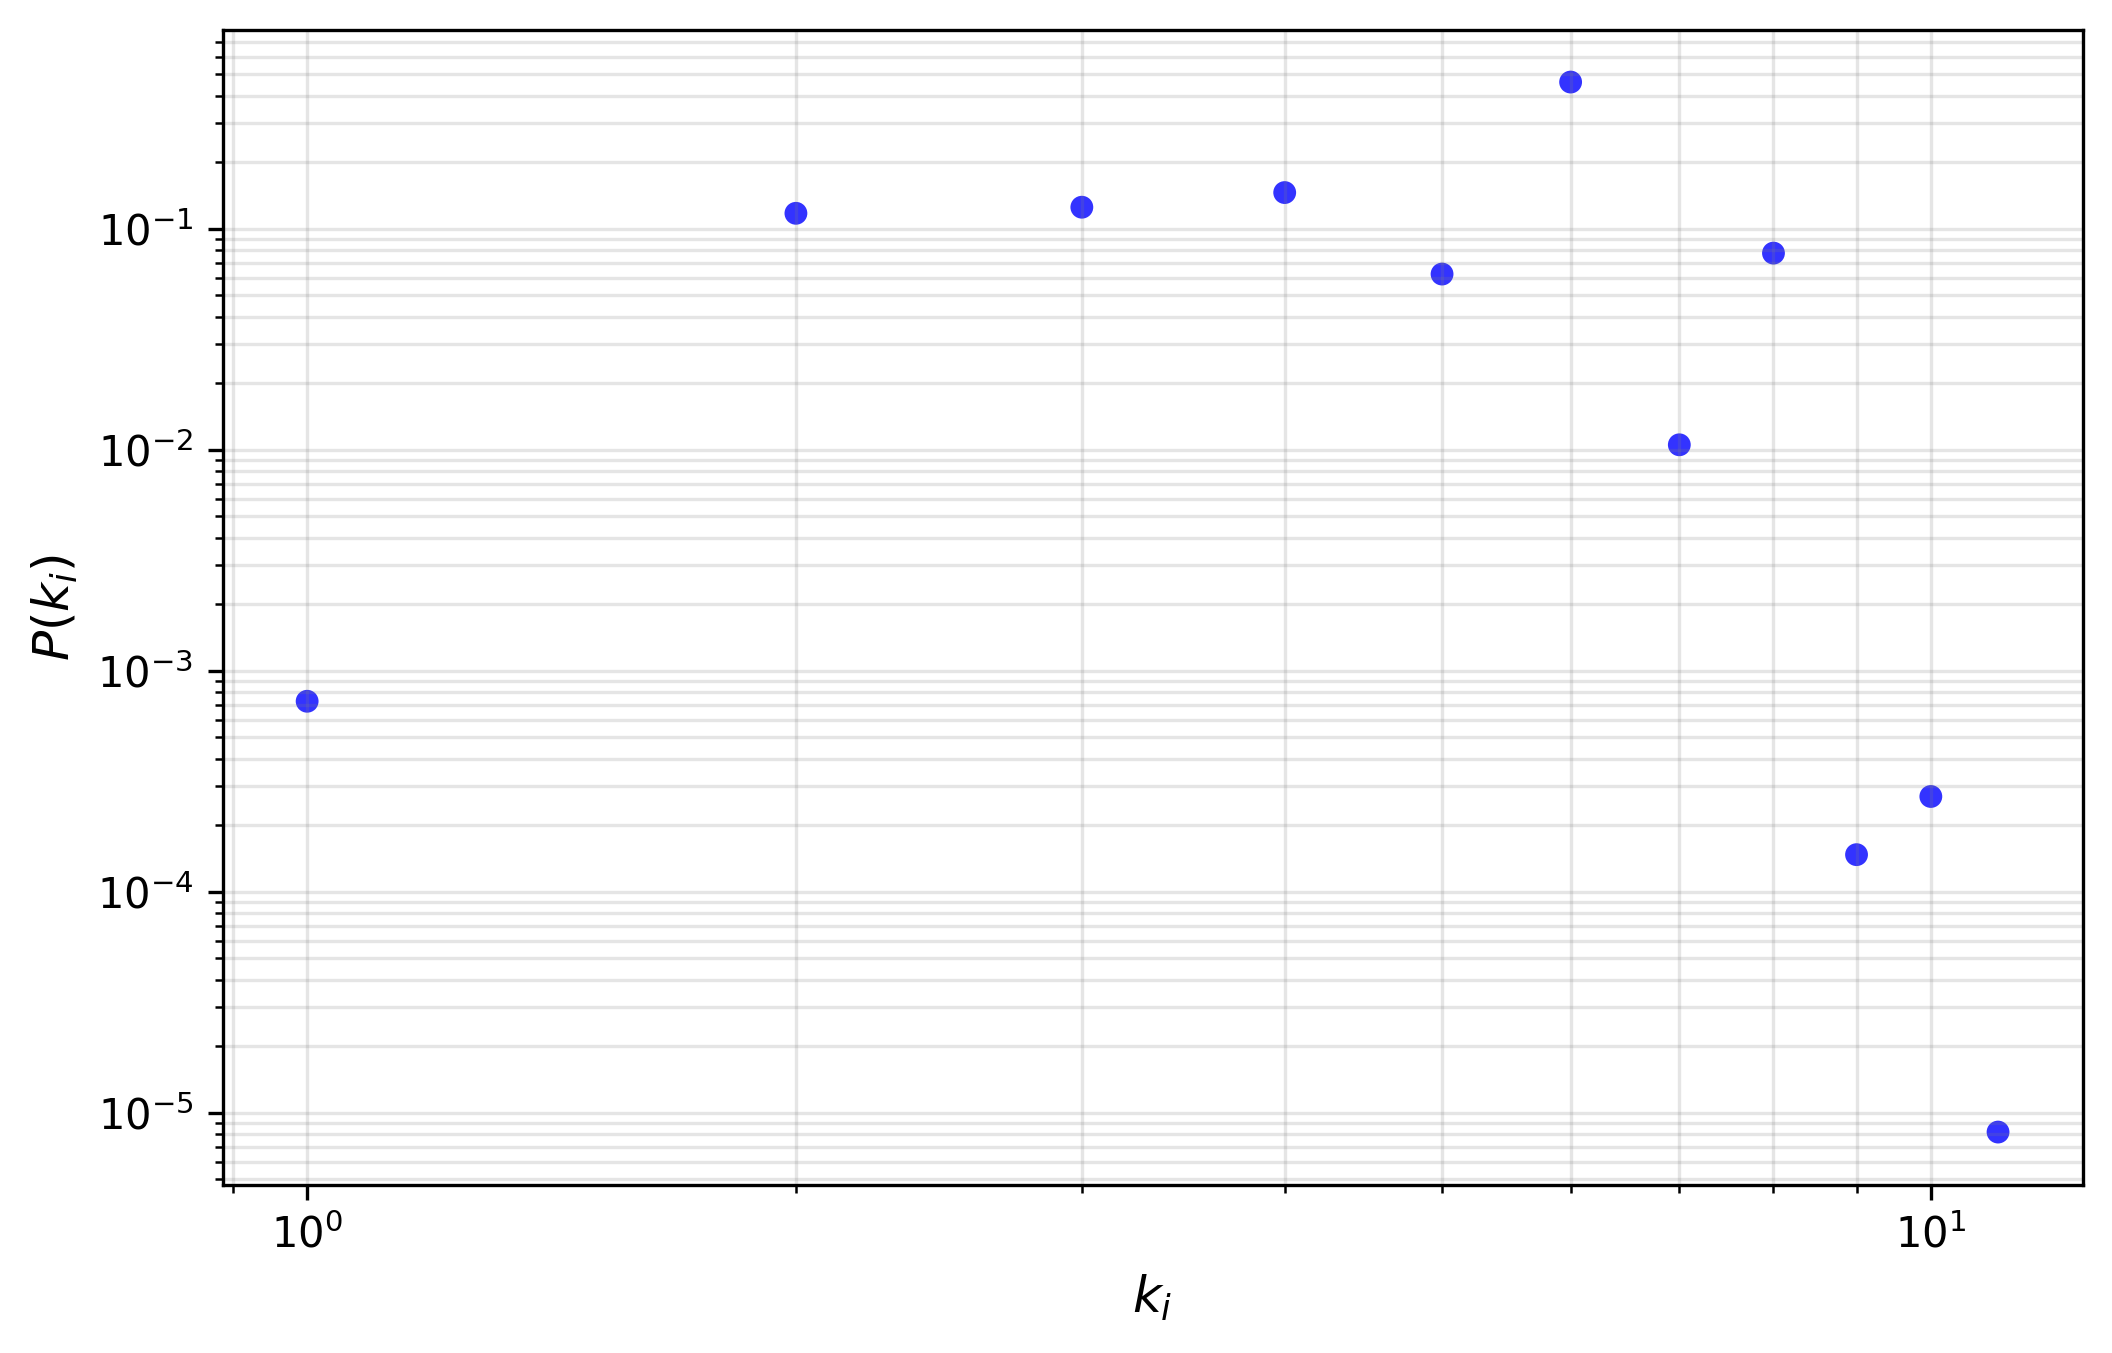
\includegraphics[width=0.7\textwidth]{../plot/degree_distribution.png}
    \caption{Distribution of $k_i$ values. Source: The Authors (2026).}
    \label{fig:ki_dist}
\end{figure}

The map in Figure \ref{fig:eij_map} shows the distribution of $e_{ij}$ values across the network. It is observed that few edges have high values of $e_{ij}$, indicating road sections that are critical routes, likely carrying high traffic volumes and concentrating flow from many origin-destination pairs. It could also indicate locations of higher vulnerability to disruptions, impacting the overall network resilience and performance.

\begin{figure}[H]
    \centering
    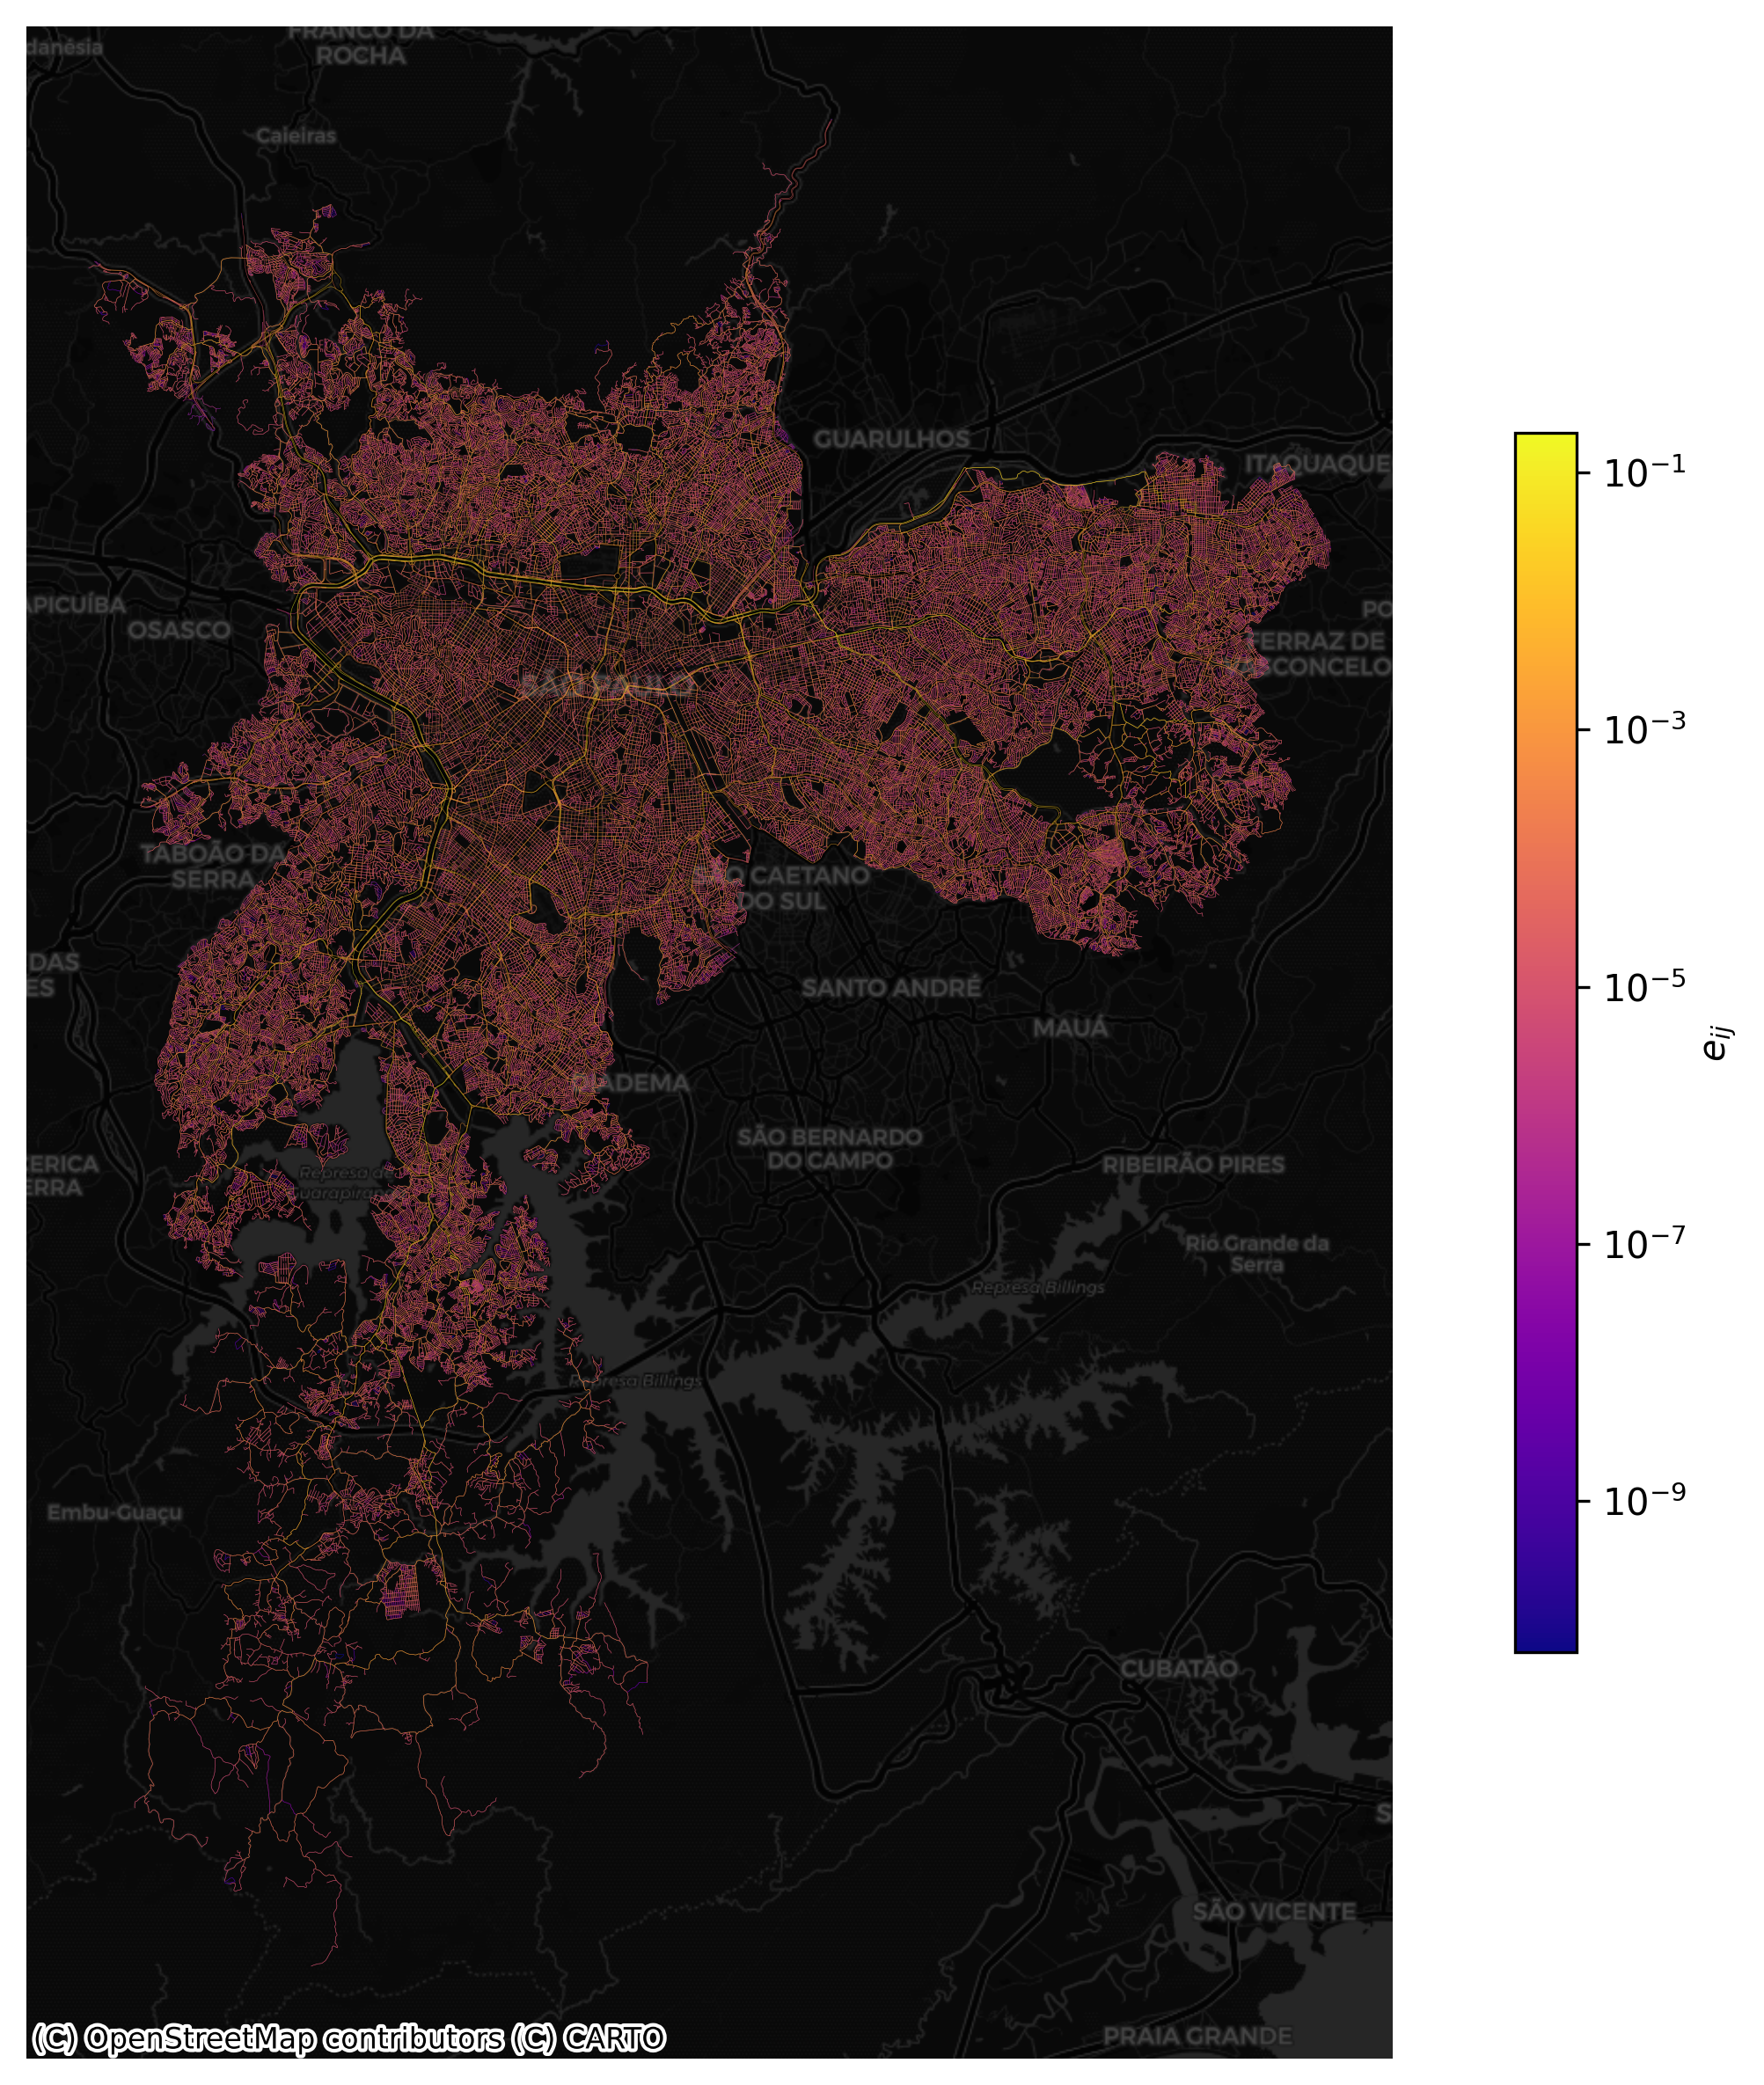
\includegraphics[width=0.7\textwidth]{../plot/edges_e_ij.png}
	\caption{Map of $e_{ij}$ results. Source: The Authors (2026).}
	\label{fig:eij_map}
\end{figure}

In Table \ref{tab:comparison}, it is possible to observe the comparison between the real São Paulo network and a theoretical random graph $G(N, p)$ to highlight the differences in their structural properties. The road network shows a higher value of $\langle c \rangle$ compared to the random graph, indicating that the real network has a strong local structure, which can be an attribute of how intersections are connected in the city (\textit{e.g.} if intersection A connects to B and to C, there is a good chance B and C are also connected by a road, especially in grid-like urban layouts.)

\begin{table}[H]
\centering
\caption{\small Comparison between the real network and the theoretical random graph $G(N, p)$.}
\label{tab:comparison}
\begin{tabular}{lrrrrrr}
\hline
Network & $N$ & $L$ & $p$ & $\langle k \rangle$ & $\langle c \rangle$ & $\langle l \rangle$ \\
\hline
Real network & 122456 & 304027 & -- & 4.9655 & 0.059600 & 132.4250 \\
$G(N, p)$ & 122456 & -- & 0.000041 & 4.9655 & 0.000041 & 7.3107 \\
\hline
\end{tabular}
\end{table}

When comparing the $\langle l \rangle$ values, it is possible to observe that the real network has an 18 times higher average path length compared to the random graph. In the random graph, any node can connect to any other, creating long-range "shortcuts" that shorten distances. A real road network is constrained by geographical distances; therefore, to go from one side of the city to the other, a road user must traverse many intermediate edges (road segments) sequentially.

\section{Conclusion}

In this work, it was possible to analyze the topological properties of the São Paulo road network. The results showed that the network distribution of degree values did not follow a power-law behavior, indicating that the degree distribution is not scale-free. Regarding edge betweenness centrality, the network presented a few edges with higher values, representing road segments that are crucial for connecting different parts of the city.

When comparing the São Paulo road network with a theoretical random graph, the results highlight the differences in their structural properties. The real network shows a higher clustering coefficient and much longer paths ($l_i$), when compared to the random graph.

Future work may explore the computation and analysis of the Vulnerability Index on edges, to better understand the robustness of the network against failures. In this work, it was not possible to compute the Vulnerability Index due to the large size of the network and the computational resources required.

%%%%%%%%%%%%%%%%%%%%%%%%%%%%%%%%%%%%%%%%%%%%%%%%%%%%%%%%%%%%%%%%%%%%%%%%
% REFS BIBLIOGRÁFICAS
% POR FAVOR, NÃO ALTERAR
%%%%%%%%%%%%%%%%%%%%%%%%%%%%%%%%%%%%%%%%%%%%%%%%%%%%%%%%%%%%%%%%%%%%%%%%
\printbibliography
%%%%%%%%%%%%%%%%%%%%%%%%%%%%%%%%%%%%%%%%%%%%%%%%%%%%%%%%%%%%%%%%%%%%%%%%

\end{document}
